\chapter{Practice: Sensor Ping}
\section*{Suggested read: Chapers~\ref{introToXBee} and~\ref{pract:simpleChat}}

In this assignment we will implement a ``ping'' over the sensor network.
We will use a script in Python to send a probe packet to a remote XBee.
Time is measured between the submission of the packet and the receipt of the acknowledgement and we present the information on the screen to the user.
To makes things more interesting, we connect an Arduino to the remote XBee that flashes a LED each time it receives a packet.
The number of times that the LED has to be flashed is included in the probe packet.

We will start by using X-CTU to flash one of the XBees as a coordinator API and the other as router API.
To prevent interference with other groups, write the PAN ID that you are going to use on the blackboard and make sure that you use a PAN ID different from other groups.
The other XBee should be configured as a Router with the same PAN ID.
It is important to set the API mode to 2 as shown in Fig. \ref{fig:ap2} for the two XBees.
Note that in the computer we are using the ``xbee'' library.


\begin{figure}[htbp]
  \centering
  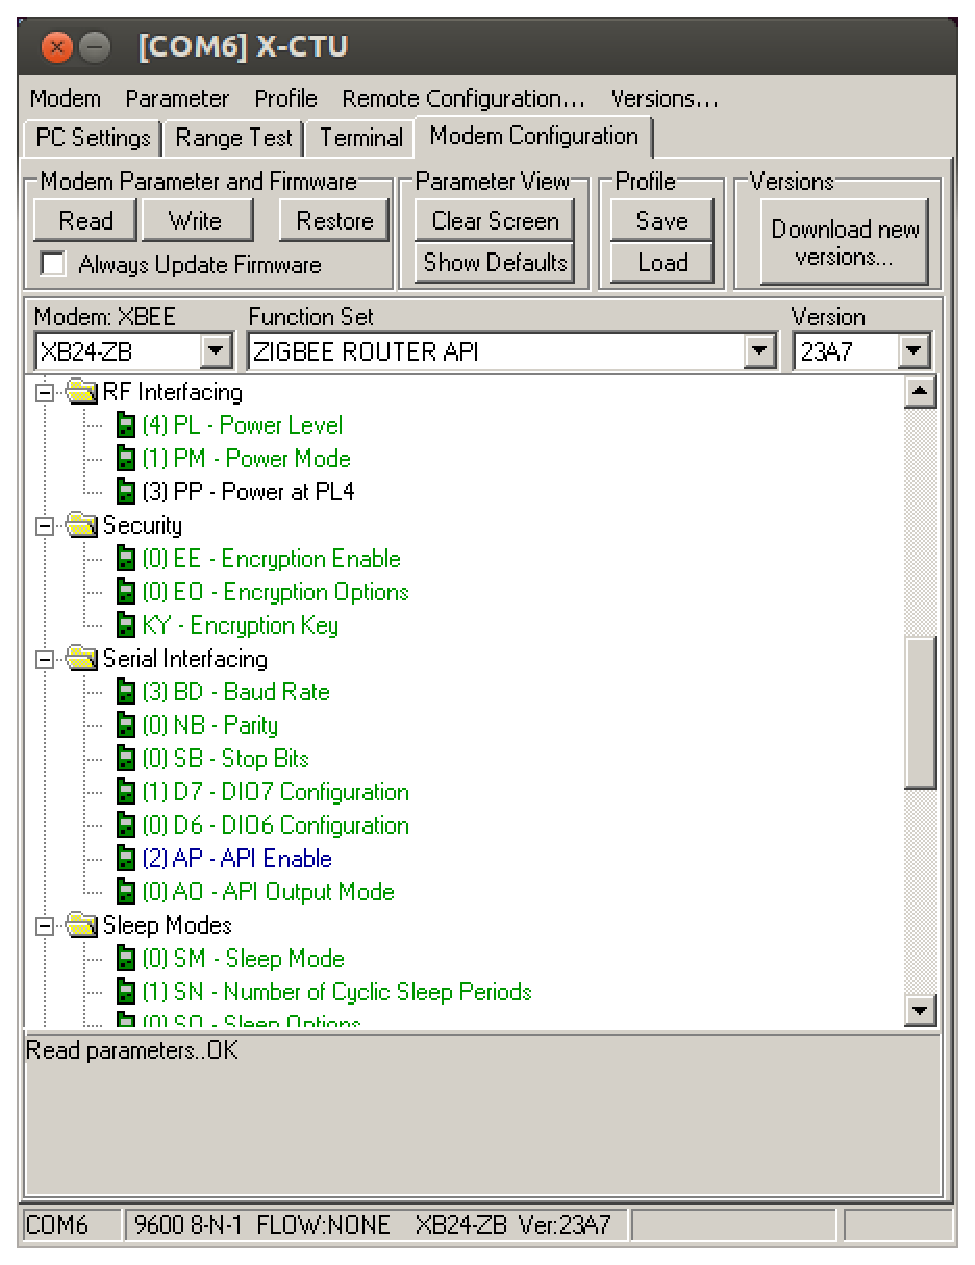
\includegraphics[width=0.9\linewidth]{figures/ap2.eps}
  \caption{Setting the API mode to 2 (AP=2)}
  \label{fig:ap2}
\end{figure}

In the computer, we will create a program that sends a ping packet to the destination every 10s (or whatever you prefer).
Replace the long destination address by the one of your XBee.
Not that the program in Listing~\ref{code:ping-sender} sends an initial probe packet to obtain the 16-bit address of the destination and then it uses this address for subsequent probes.
The time that elapses from the sending of the probe to the reception of the acknowledgement is the round-trip-time and is printed on the screen.

\begin{lstlisting} [caption = {Simple code that reads the message that arrives to the XBee.}, language = Python, label = {code:ping-sender}, numbers = left, escapeinside={@}{@}]

#! /usr/bin/python

import time
from datetime import datetime
import serial
from xbee import XBee, ZigBee

PORT = '/dev/ttyUSB0'
BAUD_RATE = 9600

# Open serial port and enable flow control
ser = serial.Serial(PORT, BAUD_RATE, bytesize=8, parity='N', stopbits=1, timeout=None, xonxoff=1, rtscts=1, dsrdtr=1)

# Create API object
xbee = ZigBee(ser,escaped=True)

DEST_ADDR_LONG = "\x00\x13\xA2\x00\x40\x8B\x3D\x91"

#part to discovery shot 16-bit address
xbee.send("tx",data="\x01",dest_addr_long=DEST_ADDR_LONG,dest_addr="\xff\xfe")
response = xbee.wait_read_frame()
shot_addr = response["dest_addr"]

# Continuously read and print packets
while True:
    try:
        print "send data"
        tstart = datetime.now()
        xbee.send("tx",data="\x03",dest_addr_long=DEST_ADDR_LONG,dest_addr=shot_addr)
        response = xbee.wait_read_frame()
        tend = datetime.now()
        print tend - tstart
        time.sleep(10)
    except KeyboardInterrupt:
        break

ser.close()

\end{lstlisting}

The provided code should work as soon as you connect the two XBees. 
You can plug the USB cables to power the two XBees and check that everything is working.
Observe the terminal on the computer with the measured delay and the RSSI indicator in the Explorer that flashes when data is transmitted.
Try to disconnect the remote XBee and observe what happens.

To make things more interesting, we will connect an Arduino to the remote XBee and flash a light each time it receives a packet.
We will use the ``xbee-arduino'' library in the Arduino as explained in Listing \ref{code:flashping}.
Each time that we receive a packet we read the first byte and flash the LED as many times as indicated in that byte.

\begin{lstlisting} [caption = {Sunset sensor}, language = C, label = {code:flashping}, numbers = left, escapeinside={@}{@}]
#include <XBee.h>

int ledPin = 13;

XBee xbee = XBee();
XBeeResponse response = XBeeResponse();
// create reusable response objects for responses we expect to handle 
ZBRxResponse rx = ZBRxResponse();

void flashLed(int pin, int times, int wait) {

    for (int i = 0; i < times; i++) {
      digitalWrite(pin, HIGH);
      delay(wait);
      digitalWrite(pin, LOW);

      if (i + 1 < times) {
        delay(wait);
      }
    }
}

void setup() {
  xbee.begin(9600);
  pinMode(ledPin, OUTPUT);
  flashLed(ledPin, 10, 50);    // sets the LED off
}

void loop() {


  // 1. This will read any data that is available:
  xbee.readPacket();
  if (xbee.getResponse().isAvailable()) {
    if (xbee.getResponse().getApiId() == ZB_RX_RESPONSE) {
      xbee.getResponse().getZBRxResponse(rx);
      //flashLed(ledPin, 1, 100);    // sets the LED off
      flashLed(ledPin, rx.getData(0), 100);    // sets the LED off
    }
  }
}
\end{lstlisting}

Program the Arduino and then connect it to the XBee. 
We are going to use the serial port to communicate with the XBee, and this same port is also used to program the Arduino.
Don't connect the Arduino/XBee serial connection until you have programmed the Arduino.
After the Arduino is programmed you can connect the TX/RX ports to the DIN/DOUT ports of the XBee.
Use the 3.3V and GND of the Arduino to power the XBee.

Test that everything is working and the Arduino flashes the number of times indicated by the computer.

\section{Next steps}

You can perform additional experiments  building on the basic examples provided here.
For example:
\begin{itemize}
\item Collaborate with another group to make ping measurements in a multi-hop setting.
\item Use a different frame identifier for each ping and compute packet loss.
\item Use broadcast messages to flash LEDs in all the Arduinos of the network.
\item Set a LED on a remote breadboard when the RTT is above a threshold.
\end{itemize}
